\documentclass[tikz,border=6pt]{standalone}
\usepackage[T1]{fontenc}
\usepackage[utf8]{inputenc}
\usepackage{amsmath,amssymb}
\usepackage{graphicx}
\usepackage{xcolor}
\usepackage{tikz}
\usepackage{pgfplots}
\usetikzlibrary{arrows.meta,backgrounds,calc,fit,matrix,positioning,shapes.geometric,shapes.misc}
\pgfplotsset{compat=1.18}

\definecolor{ink}{HTML}{1F2A30}
\definecolor{slate}{HTML}{5C6A73}
\definecolor{teal}{HTML}{2B7A8C}
\definecolor{brick}{HTML}{B6514A}
\definecolor{gold}{HTML}{C9951A}
\definecolor{sage}{HTML}{6B8C6E}
\definecolor{sky}{HTML}{5E8CC0}
\definecolor{paperbg}{HTML}{FBF7EF}
\definecolor{panel}{HTML}{F2ECE2}
\definecolor{linegray}{HTML}{D4CBBE}
\definecolor{softgreen}{HTML}{DCEBD8}
\definecolor{softred}{HTML}{F4DAD5}
\definecolor{softblue}{HTML}{DCE8F4}
\definecolor{softgold}{HTML}{F4E7C6}

\tikzset{
  figtitle/.style={font=\bfseries\Large, text=ink},
  flowbox/.style={
    draw=ink,
    rounded corners=6pt,
    line width=0.9pt,
    fill=paperbg,
    minimum height=1.35cm,
    minimum width=3.1cm,
    align=center,
    text=ink,
    inner sep=7pt
  },
  sourcebox/.style={flowbox, fill=softblue, draw=sky},
  missingbox/.style={flowbox, fill=softred, draw=brick, dashed},
  gatebox/.style={flowbox, fill=softgold, draw=gold!90!ink, text width=3.7cm},
  successbox/.style={flowbox, fill=softgreen, draw=sage, text width=3.8cm},
  card/.style={
    draw=ink,
    rounded corners=6pt,
    line width=0.8pt,
    fill=paperbg,
    text=ink,
    text width=4.0cm,
    align=left,
    inner sep=7pt
  },
  promote/.style={card, fill=softgreen, draw=sage},
  hold/.style={card, fill=softgold, draw=gold!80!ink},
  retire/.style={card, fill=softred, draw=brick},
  headercard/.style={
    draw=ink,
    rounded corners=7pt,
    line width=1.0pt,
    fill=panel,
    text=ink,
    font=\bfseries\large,
    minimum width=4.3cm,
    minimum height=1.0cm,
    align=center
  },
  figarrow/.style={-Latex, line width=1.05pt, draw=slate},
  stagearrow/.style={-Latex, line width=1.2pt, draw=ink},
  faintarrow/.style={-Latex, line width=0.9pt, draw=linegray},
  ann/.style={font=\footnotesize, text=slate, align=left},
  smallann/.style={font=\scriptsize, text=slate, align=left},
  metric/.style={
    draw=ink,
    rounded corners=6pt,
    line width=0.8pt,
    fill=white,
    text=ink,
    text width=3.6cm,
    align=left,
    inner sep=7pt
  },
  legendlabel/.style={font=\small, text=ink}
}

\pgfplotsset{
  archivara axis/.style={
    width=15cm,
    height=8.6cm,
    axis line style={draw=ink, line width=0.9pt},
    tick style={draw=ink},
    ticklabel style={font=\small, text=ink},
    label style={font=\small, text=ink},
    grid=both,
    major grid style={draw=linegray, line width=0.35pt},
    minor grid style={draw=linegray!60, line width=0.2pt},
    legend style={
      draw=none,
      fill=none,
      font=\small,
      text=ink,
      /tikz/every even column/.append style={column sep=0.5cm}
    },
    clip=false
  }
}


\begin{document}
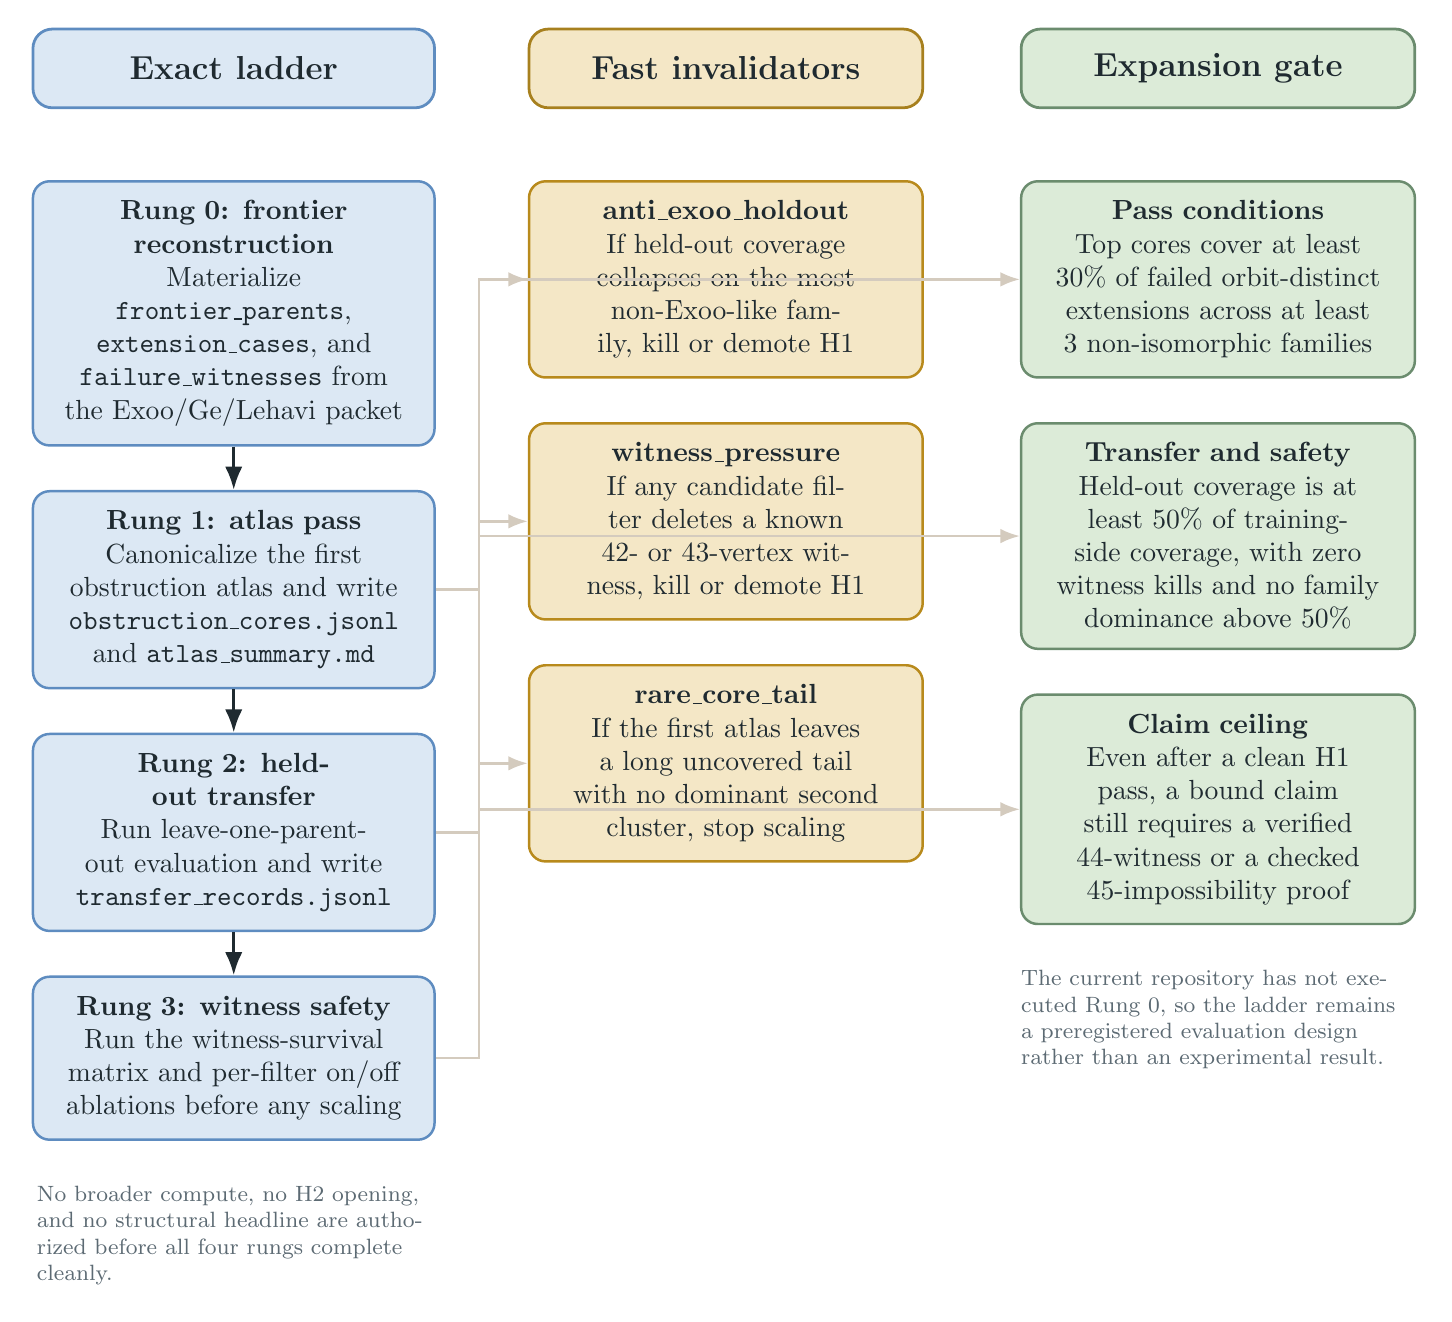
\begin{tikzpicture}[node distance=0.9cm and 1.1cm]
  \node[headercard, minimum width=5.1cm, fill=softblue, draw=sky] (title1) at (0,0) {Exact ladder};
  \node[headercard, minimum width=5.0cm, fill=softgold, draw=gold!80!ink] (title2) at (6.25,0) {Fast invalidators};
  \node[headercard, minimum width=5.0cm, fill=softgreen, draw=sage] (title3) at (12.5,0) {Expansion gate};

  \node[sourcebox, below=0.9cm of title1, minimum width=5.1cm, text width=4.45cm] (r0)
    {\textbf{Rung 0: frontier reconstruction}\\Materialize \texttt{frontier\_parents}, \texttt{extension\_cases}, and \texttt{failure\_witnesses} from the Exoo/Ge/Lehavi packet};
  \node[sourcebox, below=0.55cm of r0, minimum width=5.1cm, text width=4.45cm] (r1)
    {\textbf{Rung 1: atlas pass}\\Canonicalize the first obstruction atlas and write \texttt{obstruction\_cores.jsonl} and \texttt{atlas\_summary.md}};
  \node[sourcebox, below=0.55cm of r1, minimum width=5.1cm, text width=4.45cm] (r2)
    {\textbf{Rung 2: held-out transfer}\\Run leave-one-parent-out evaluation and write \texttt{transfer\_records.jsonl}};
  \node[sourcebox, below=0.55cm of r2, minimum width=5.1cm, text width=4.45cm] (r3)
    {\textbf{Rung 3: witness safety}\\Run the witness-survival matrix and per-filter on/off ablations before any scaling};

  \draw[stagearrow] (r0) -- (r1);
  \draw[stagearrow] (r1) -- (r2);
  \draw[stagearrow] (r2) -- (r3);

  \node[gatebox, below=0.9cm of title2, minimum width=5.0cm, text width=4.25cm] (f1)
    {\textbf{anti\_exoo\_holdout}\\If held-out coverage collapses on the most non-Exoo-like family, kill or demote H1};
  \node[gatebox, below=0.55cm of f1, minimum width=5.0cm, text width=4.25cm] (f2)
    {\textbf{witness\_pressure}\\If any candidate filter deletes a known $42$- or $43$-vertex witness, kill or demote H1};
  \node[gatebox, below=0.55cm of f2, minimum width=5.0cm, text width=4.25cm] (f3)
    {\textbf{rare\_core\_tail}\\If the first atlas leaves a long uncovered tail with no dominant second cluster, stop scaling};

  \node[successbox, below=0.9cm of title3, minimum width=5.0cm, text width=4.2cm] (g1)
    {\textbf{Pass conditions}\\Top cores cover at least $30\%$ of failed orbit-distinct extensions across at least $3$ non-isomorphic families};
  \node[successbox, below=0.55cm of g1, minimum width=5.0cm, text width=4.2cm] (g2)
    {\textbf{Transfer and safety}\\Held-out coverage is at least $50\%$ of training-side coverage, with zero witness kills and no family dominance above $50\%$};
  \node[successbox, below=0.55cm of g2, minimum width=5.0cm, text width=4.2cm] (g3)
    {\textbf{Claim ceiling}\\Even after a clean H1 pass, a bound claim still requires a verified $44$-witness or a checked $45$-impossibility proof};

  \draw[faintarrow] (r1.east) -- ++(0.55,0) |- (f1.west);
  \draw[faintarrow] (r2.east) -- ++(0.55,0) |- (f2.west);
  \draw[faintarrow] (r3.east) -- ++(0.55,0) |- (f3.west);

  \draw[faintarrow] (r1.east) -- ++(0.55,0) |- (g1.west);
  \draw[faintarrow] (r2.east) -- ++(0.55,0) |- (g2.west);
  \draw[faintarrow] (r3.east) -- ++(0.55,0) |- (g3.west);

  \node[ann, below=0.45cm of r3, text width=5.0cm]
    {No broader compute, no H2 opening, and no structural headline are authorized before all four rungs complete cleanly.};
  \node[ann, below=0.45cm of g3, text width=5.0cm]
    {The current repository has not executed Rung 0, so the ladder remains a preregistered evaluation design rather than an experimental result.};
\end{tikzpicture}
\end{document}
